\chapter{Convex Polytopes}

\scribe{Cecilia Gir\'on}
 
A convex polytope can be defined in two different ways:
\begin{enumerate}
\item[-] \textit{$V$-polytope} (discrete geometry): is the convex hull of the finite non-empty point set in $\mathbf{R}^d$.
\item[-]\textit{$H$-polytope} (linear/integer optimization): An $H$-polyhedron is an intersection of a finite number of linear half spaces in some $\mathbf{R}^d$, if non-empty. And an $H$-polytope is a bounded $H$-polyhedron. 
\end{enumerate}
\bigskip
\section{Faces}
One of the properties studied about polytopes is their faces. A \textbf{face} $F$ of a polytope $P$ is a set of the form:
\[F = \{x\in \mathbb{R}^d: <a,x> = n\}\cap P\]
where $a\in (\mathbb{R}^d)^*$ (dual space), $b\in\mathbb{R}$ and $P\subseteq\{x\in\mathbb{R}^d: <a,x> \leq b \}\longleftrightarrow$ The inequality $<a,x> \leq b$ is valid for $P$. Notice that $P$ is actually a face of itself. 

We can also study the dimension $\dim F$ of a face. Let $P$ be a $d$ dimensional polytope, then if a face $F$ of $P$ has dimension:
\begin{itemize}
\item[i)] $d -1$, it is called a \textbf{facet}.
\item[ii)] $d -2$, it is called a \textbf{ridge}.
\item[iii)] $1$, it is called an \textbf{edge}.
\item[iv)] $0$, it is called a \textbf{vertex}.
\item[v)] $ -1$ then $F=\emptyset$.
\end{itemize}

The partially ordered set of all faces  $\mathcal{F}(P)$ of a convex polytope $P$ forms a Eulerian lattice called \textbf{face lattice}. The face lattice can be used, for instance, to count the number of faces of same dimension:
\[f_i = \# \{ \mbox{ faces } F \mbox{ of } P \mbox{ with } \dim F=i\} \label{eq1}\]

\bigskip

\textsc{Example}. Let $P$ be a cube in two dimensions, so a square. Notice that $\dim P = 2$, for every edge $ij\in P$ $\dim(ij) = 1$ and for every vertex $i$ $\dim i= 0$, for $i,j= 1, 2 , 3,4$ and $i\neq j$. With this information we can construct the face lattice and study some properties of $P$.

\begin{figure}[h!]
\begin{minipage}[t]{0.4\textwidth}
   \vspace{30pt}
   \hspace{20pt}

\begin{picture}(100,100)
\put(115,0){4}
\put(0,1){3}
\put(0,100){1}
\put(115,100){2}
\put(8,105){\textbullet}
\put(108,105){\textbullet}
\put(8,8){\textbullet}
\put(108,8){\textbullet}
\multiput(10,10)(100,0){2}{\line(0,100){100}}
\multiput(10,10)(0,100){2}{\line(100,0){100}}
\end{picture}

\end{minipage}
  \hfill
\begin{minipage}[t]{0.6\textwidth}
      \vspace{0pt}
      \hspace{-100pt}
\[
\xymatrix{
& & P\ar[dr]\ar[drr]\ar[dl]\ar[dll] & & & f_2 = 1 \\
13\ar[d]\ar[drrrr]  & 12\ar[d]\ar[dl]&  & 24\ar[d]\ar[dll] & 34\ar[d]\ar[dl] & f_ 1 = 4\\
1\ar[drr]  & 2\ar[dr]&  & 3\ar[dl] & 4\ar[dll] & f_0=4\\
 & & \emptyset & & & F_{-1}=1
 }
\]
\end{minipage}
\end{figure} 


\begin{flushright}
$\clubsuit$
\end{flushright}

\bigskip
\textsc{Example}.Let's study now the dimension of the faces of a hypercube of dimension d $\square ^d = \{ x\in\mathbb{R}^d: -1\leq x_i\leq 1, i=1,\cdots, d\}$: $f_{-1}(\square ^d) = 1, f_{0}(\square ^d) = 2^d,f_{d-1}(\square ^d) = 2d $ and $f_{d}(\square ^d) = 1$. Notice that the radius $r$ from the center of the cube to one of its vertices is $r=\sqrt{d}-1$, thus the exterior circus of the polytope has radio $r$ and the interior radio 1. 
\bigskip



\begin{tabular}{| c | c | c | c | c | c | c | c | c |}
  \hline                        
  d & 2 & 3 & 4 & 5 & $\cdots$ & 100 & $\cdots$ & $10^{100}$ \\
  \hline 
 $r=\sqrt{d}-1$ & $\sqrt{2}-1$ & $\sqrt{3}-1$ & $1$ & $\sqrt{5}-1$ & $\cdots$ & 9  & $\cdots$ & $10^{50}-1$ \\
  \hline  
  $f_0$ & $4$ & $8$ & $16$  & $32$ &  $\cdots$ & $2^{100}$ &  $\cdots$ & $2^{10^{100}}$ \\
  \hline
  $f_{1}$ & $4$ & $6$ & $8$  & $10$ &  $\cdots$ & $200$ &  $\cdots$ & $2\cdot 10^{100}$ \\
  \hline  
\end{tabular}

\begin{flushright}
$\clubsuit$
\end{flushright}

\bigskip

An other property that can be studied about the faces of convex polytopes is whether they are a simplex or not. Let $P$ be a polytope such that $\dim P = d$ and $\mathcal{F}(p) = k+1$. It is said to be \textbf{simplicial} if it is $k$-simplex, i.e. if each of its faces is a simplex; and it is called \textbf{simple} if each of its vertices is contained in exactly $d$ faces where $\dim P =d$.

\bigskip
\subsection{Exercises done during the lecture 8/11/2013. Each one includes one}

\begin{description}
\item [Alex Alvarez.] The set of vertices is the following:
\begin{verbatim}
(1 : -1 : -1 : -1 : 0 : 0)
(1 : 1 : -1 : -1 : 0 : 0)
(1 : -1 : 1 : -1 : 0 : 0)
(1 : 1 : 1 : -1 : 0 : 0)
(1 : 0 : 0 : 1 : 0 : 0)
(1 : 0 : 0 : 1 : 1 : 0)
(1 : 0 : 0 : 1 : 0 : 1)
\end{verbatim}
If we look at the first four vertices, they form a square in $\mathbb{R}^3$ and together with the next vertex, a pyramid. The other two points have non-zero coordinates in dimension 4 and 5.

If we put these points in Polymake:
\begin{verbatim}
polytope > $p = new Polytope<Rational>;

polytope > $p->POINTS = <<".";
polytope (2)> 1 -1 -1 -1 0 0
polytope (3)> 1 1 -1 -1 0 0
polytope (4)> 1 -1 1 -1 0 0
polytope (5)> 1 1 1 -1 0 0
polytope (6)> 1 0 0 1 0 0
polytope (7)> 1 0 0 1 1 0
polytope (8)> 1 0 0 1 0 1
polytope (9)> .
\end{verbatim}

Thus, we can use the program to see the number of facets and the vertices in each facet:

\begin{verbatim}
polytope > print $p->N_FACETS;
polymake: used package cddlib
  Implementation of the double description method of Motzkin et al.
    Copyright by Komei Fukuda.
      http://www.ifor.math.ethz.ch/~fukuda/cdd_home/cdd.html

      polymake: used package lrslib
        Implementation of the reverse search algorithm of Avis and Fukuda.
          Copyright by David Avis.
            http://cgm.cs.mcgill.ca/~avis/lrs.html

            7
            polytope > print $p->POINTS_IN_FACETS;
            {0 2 4 5 6}
            {0 1 4 5 6}
            {1 3 4 5 6}
            {2 3 4 5 6}
            {0 1 2 3 5 6}
            {0 1 2 3 4 6}
            {0 1 2 3 4 5}
            \end{verbatim}

            If we focus now in the graph of the polytope, we can check the number of edges and we can also see it:
            \begin{verbatim}
            polytope > print $p->GRAPH->N_NODES;
            7
            polytope > print $p->GRAPH->N_EDGES;
            19
            polytope > print $p->GRAPH->VISUAL;
            \end{verbatim}

            \begin{figure}[!h]
            \centering 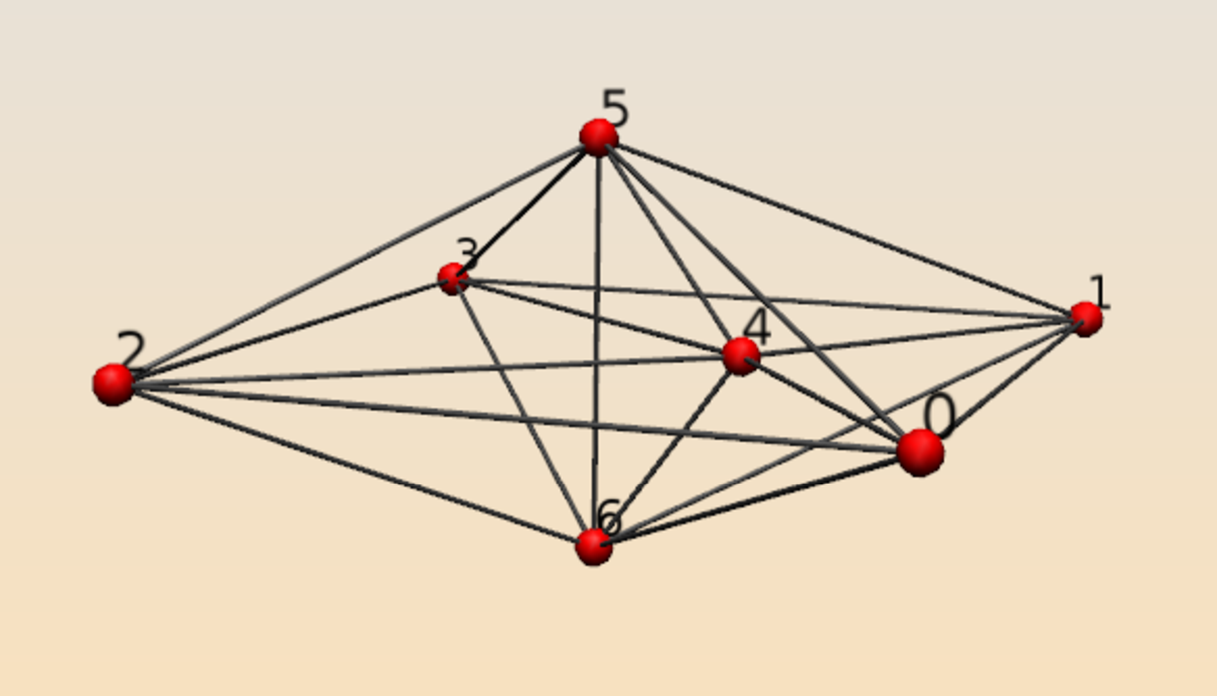
\includegraphics[width=\textwidth]{alex-alvarez-exercise-graph}
            \caption{The graph of the polytope}
            \end{figure}
            Therefore, we can see that the last two vertices are not connected, but they are connected to all the other vertices.
\item[Exercise ?? (team members)] 
\end{description}



% Local Variables: 
% mode: latex
% TeX-master: "dag-upc"
% End: 
